\documentclass[a4paper,12pt]{article}
\usepackage[utf8]{inputenc}
\usepackage{amsmath}
\usepackage{graphicx}
\usepackage{booktabs}
\usepackage{geometry}
\geometry{margin=2.5cm}
\title{Modelagem Matemática da Queda Livre}
\author{Seu Nome}
\date{\today}

\begin{document}
\maketitle

\section{Introdução}
A queda livre é um fenômeno clássico da física, modelado por equações diferenciais. Este relatório apresenta a modelagem computacional da queda livre, análise de resultados e comparação com a solução analítica, incluindo o efeito da resistência do ar.

\section{Parâmetros Utilizados}
\begin{itemize}
	\item Altura inicial: $H = 100.0$ m
	\item Velocidade inicial: $V = 0.0$ m/s
	\item Gravidade: $g = 9.81$ m/s$^2$
	\item Passos de tempo testados: $\Delta t = 1.0$, $0.5$, $0.1$, $0.01$ s
\end{itemize}

\section{Modelo Computacional}
O método de Euler foi utilizado para resolver numericamente as equações da queda livre. Os dados de entrada e saída foram salvos em arquivos txt e os gráficos gerados estão apresentados a seguir.

\section{Resultados Numéricos}
\subsection{Tabela: Simulação para $\Delta t = 0.1$ s}
\begin{tabular}{cccc}
\toprule
Tempo (s) & Posição (m) & Velocidade (m/s) \\
\midrule
0.0000 & 100.0000 & 0.0000 \\
0.1000 & 100.0000 & -0.9810 \\
0.2000 & 99.9019 & -1.9620 \\
0.3000 & 99.7057 & -2.9430 \\
0.4000 & 99.4114 & -3.9240 \\
0.5000 & 99.0190 & -4.9050 \\
0.6000 & 98.5285 & -5.8860 \\
0.7000 & 97.9399 & -6.8670 \\
0.8000 & 97.2532 & -7.8480 \\
0.9000 & 96.4684 & -8.8290 \\
1.0000 & 95.5855 & -9.8100 \\
\bottomrule
\end{tabular}

\subsection{Gráficos}
\begin{figure}[h!]
	\centering
	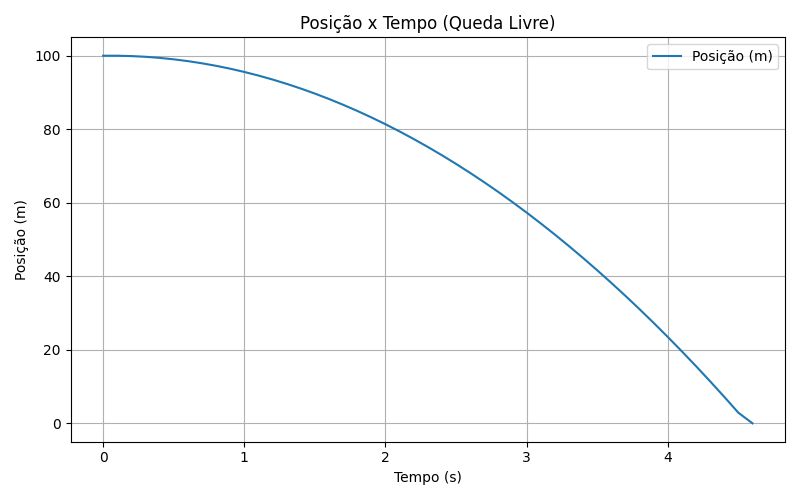
\includegraphics[width=0.7\textwidth]{../src/saida/grafico_posicao_tempo.png}
	\caption{Posição x Tempo (Queda Livre)}
\end{figure}

\begin{figure}[h!]
	\centering
	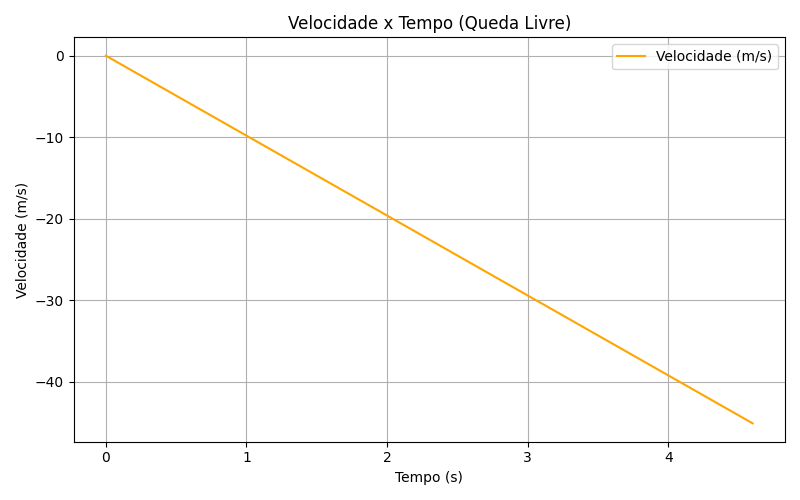
\includegraphics[width=0.7\textwidth]{../src/saida/grafico_velocidade_tempo.png}
	\caption{Velocidade x Tempo (Queda Livre)}
\end{figure}

\begin{figure}[h!]
	\centering
	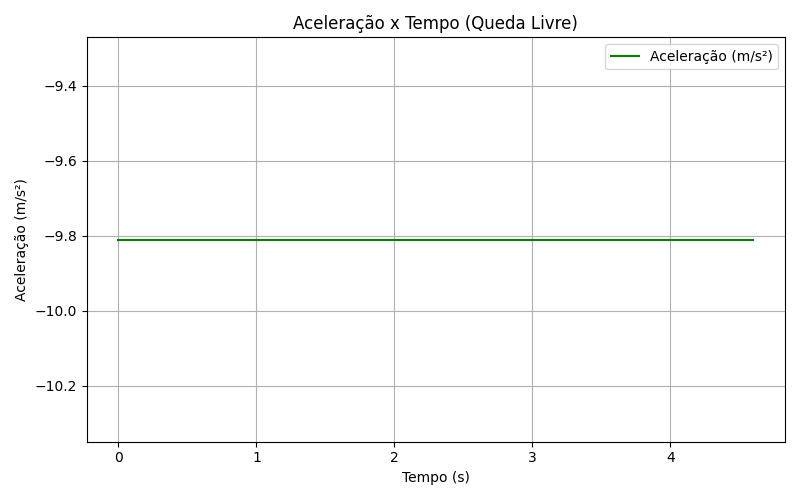
\includegraphics[width=0.7\textwidth]{../src/saida/grafico_aceleracao_tempo.png}
	\caption{Aceleração x Tempo (Queda Livre)}
\end{figure}

\section{Acurácia do Método}
\subsection{Comparação do tempo de queda}
\begin{tabular}{cccc}
\toprule
$\Delta t$ (s) & Tempo simulado (s) & Tempo analítico (s) & Erro absoluto (s) \\
\midrule
1.0 & 6.000000 & 4.515236 & 1.484764 \\
0.5 & 5.000000 & 4.515236 & 0.484764 \\
0.1 & 4.600000 & 4.515236 & 0.084764 \\
0.01 & 4.530000 & 4.515236 & 0.014764 \\
\bottomrule
\end{tabular}

\begin{figure}[h!]
	\centering
	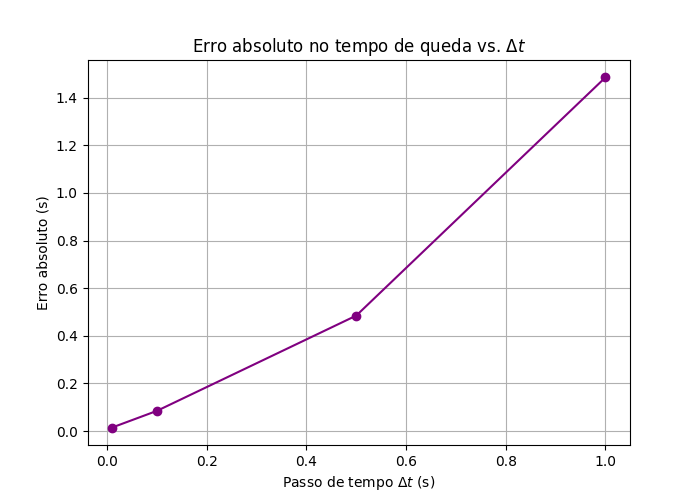
\includegraphics[width=0.7\textwidth]{../src/saida/grafico_erro_absoluto_vs_dt.png}
	\caption{Erro absoluto no tempo de queda em função de $\Delta t$}
\end{figure}

\section{Efeito da Resistência do Ar}
\subsection{Tabela: Simulação com resistência ($c=0.1$)}
\begin{tabular}{cccc}
\toprule
Tempo (s) & Posição (m) & Velocidade (m/s) \\
\midrule
0.0000 & 100.0000 & 0.0000 \\
0.1000 & 100.0000 & -0.9810 \\
0.2000 & 99.9019 & -1.9718 \\
0.3000 & 99.7047 & -2.9725 \\
0.4000 & 99.4075 & -3.9833 \\
0.5000 & 99.0091 & -5.0041 \\
0.6000 & 98.5087 & -6.0351 \\
0.7000 & 97.9052 & -7.0765 \\
0.8000 & 97.1976 & -8.1282 \\
0.9000 & 96.3847 & -9.1905 \\
1.0000 & 95.4657 & -10.2634 \\
\bottomrule
\end{tabular}

\begin{figure}[h!]
	\centering
	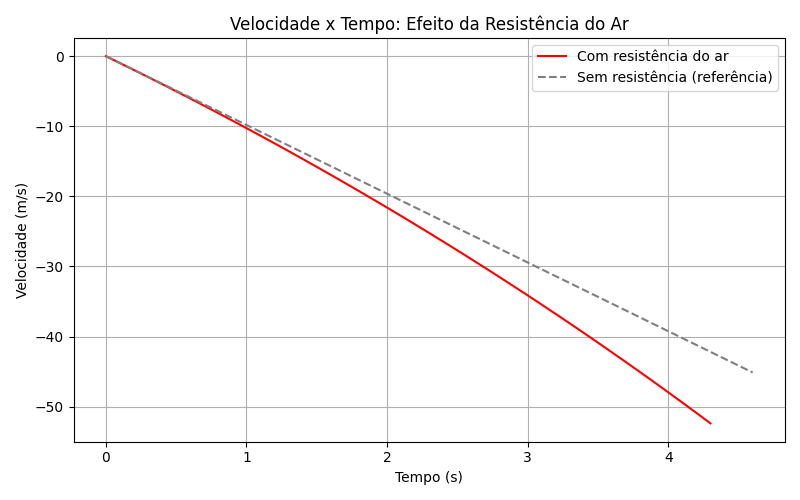
\includegraphics[width=0.7\textwidth]{../src/saida/grafico_velocidade_resistencia.png}
	\caption{Velocidade x Tempo: Efeito da Resistência do Ar}
\end{figure}

\section{Comparação: Posição x Tempo para Diferentes $\Delta t$}
\begin{figure}[h!]
	\centering
	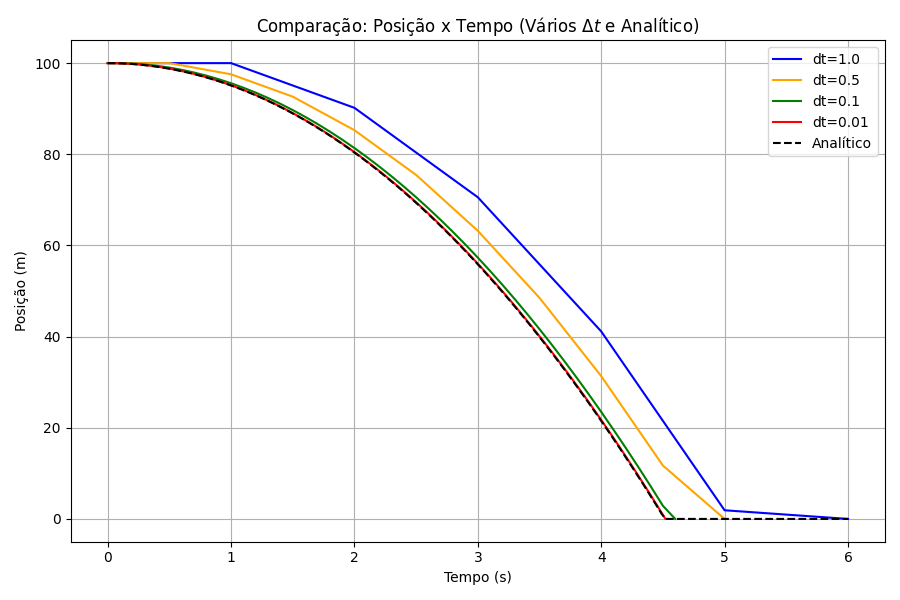
\includegraphics[width=0.8\textwidth]{../src/saida/grafico_comparacao_posicao_tempo.png}
	\caption{Comparação das curvas de posição para diferentes $\Delta t$ e solução analítica}
\end{figure}

\section{Conclusão}
O método de Euler permite simular a queda livre com boa aproximação, especialmente para passos de tempo pequenos. A inclusão da resistência do ar mostra a importância de considerar forças adicionais para maior realismo. O erro diminui conforme $\Delta t$ se reduz, validando a eficiência do método numérico.

\end{document}
